
\documentclass[]{article}
\usepackage{graphicx}

% Title Page
\title{}
\author{}


\begin{document}

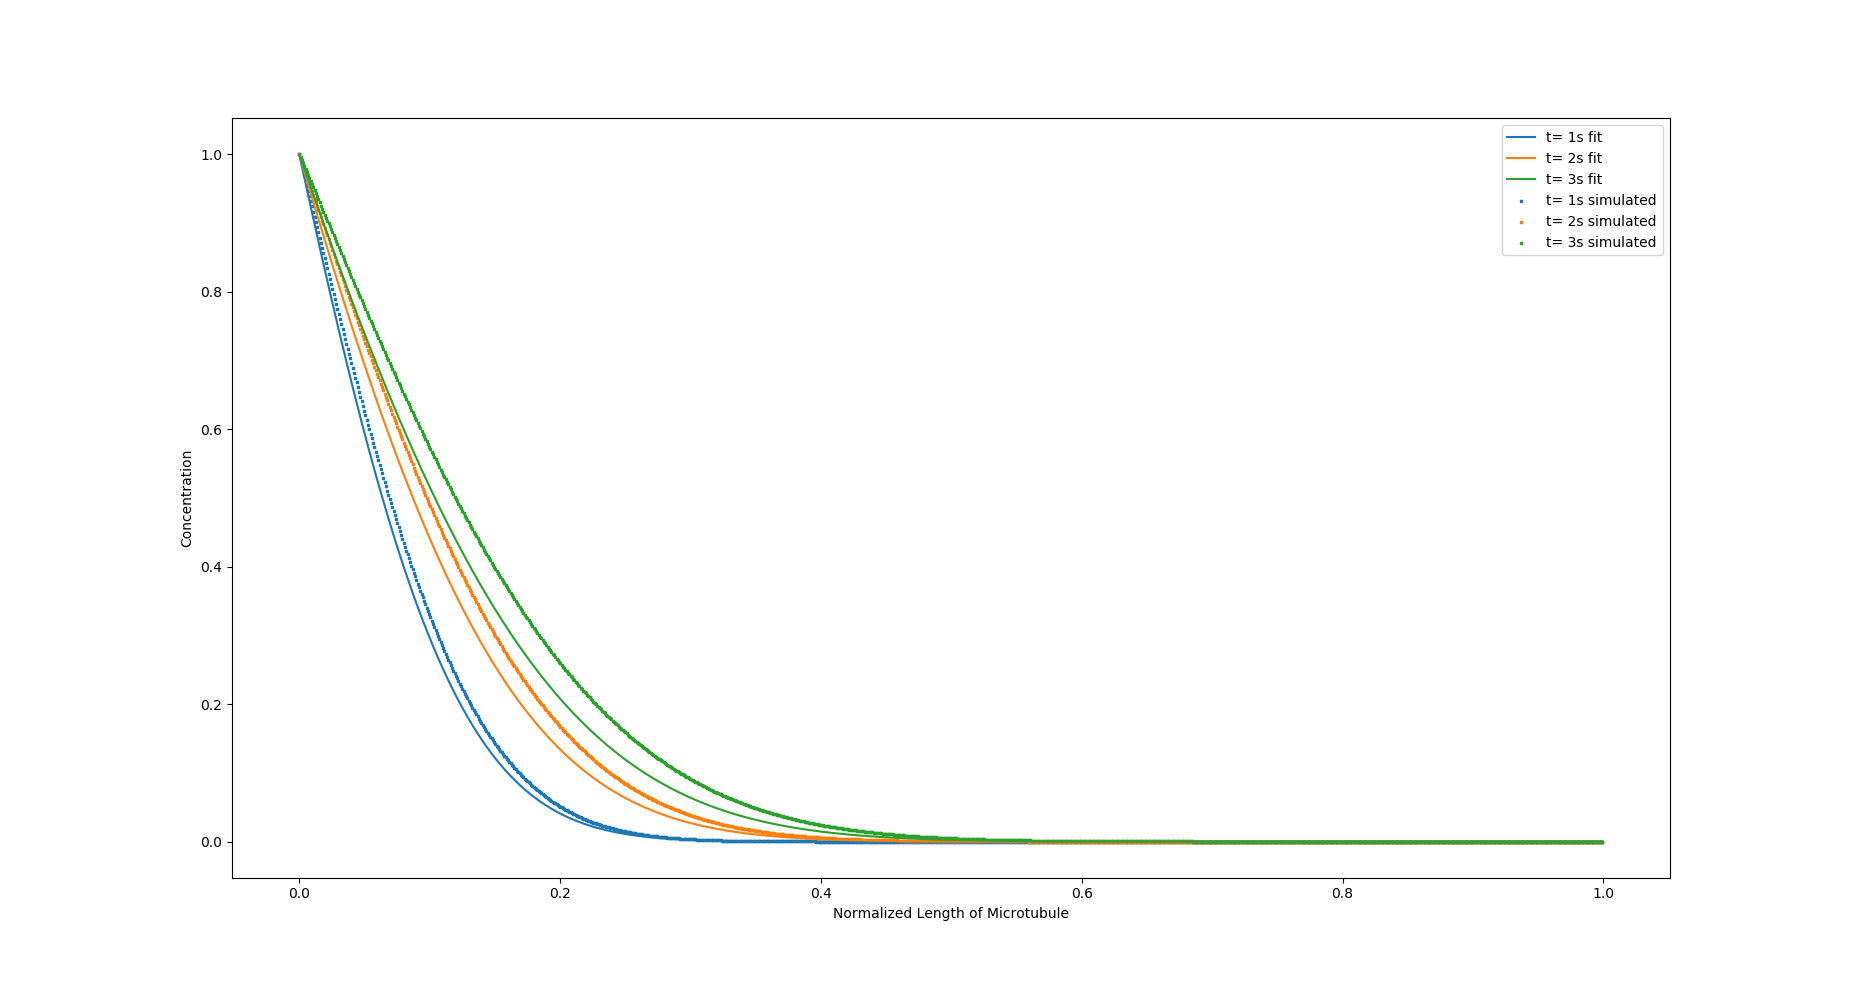
\includegraphics[width=\textwidth]{OccupationFitsWithSteadyStateMultiplication}
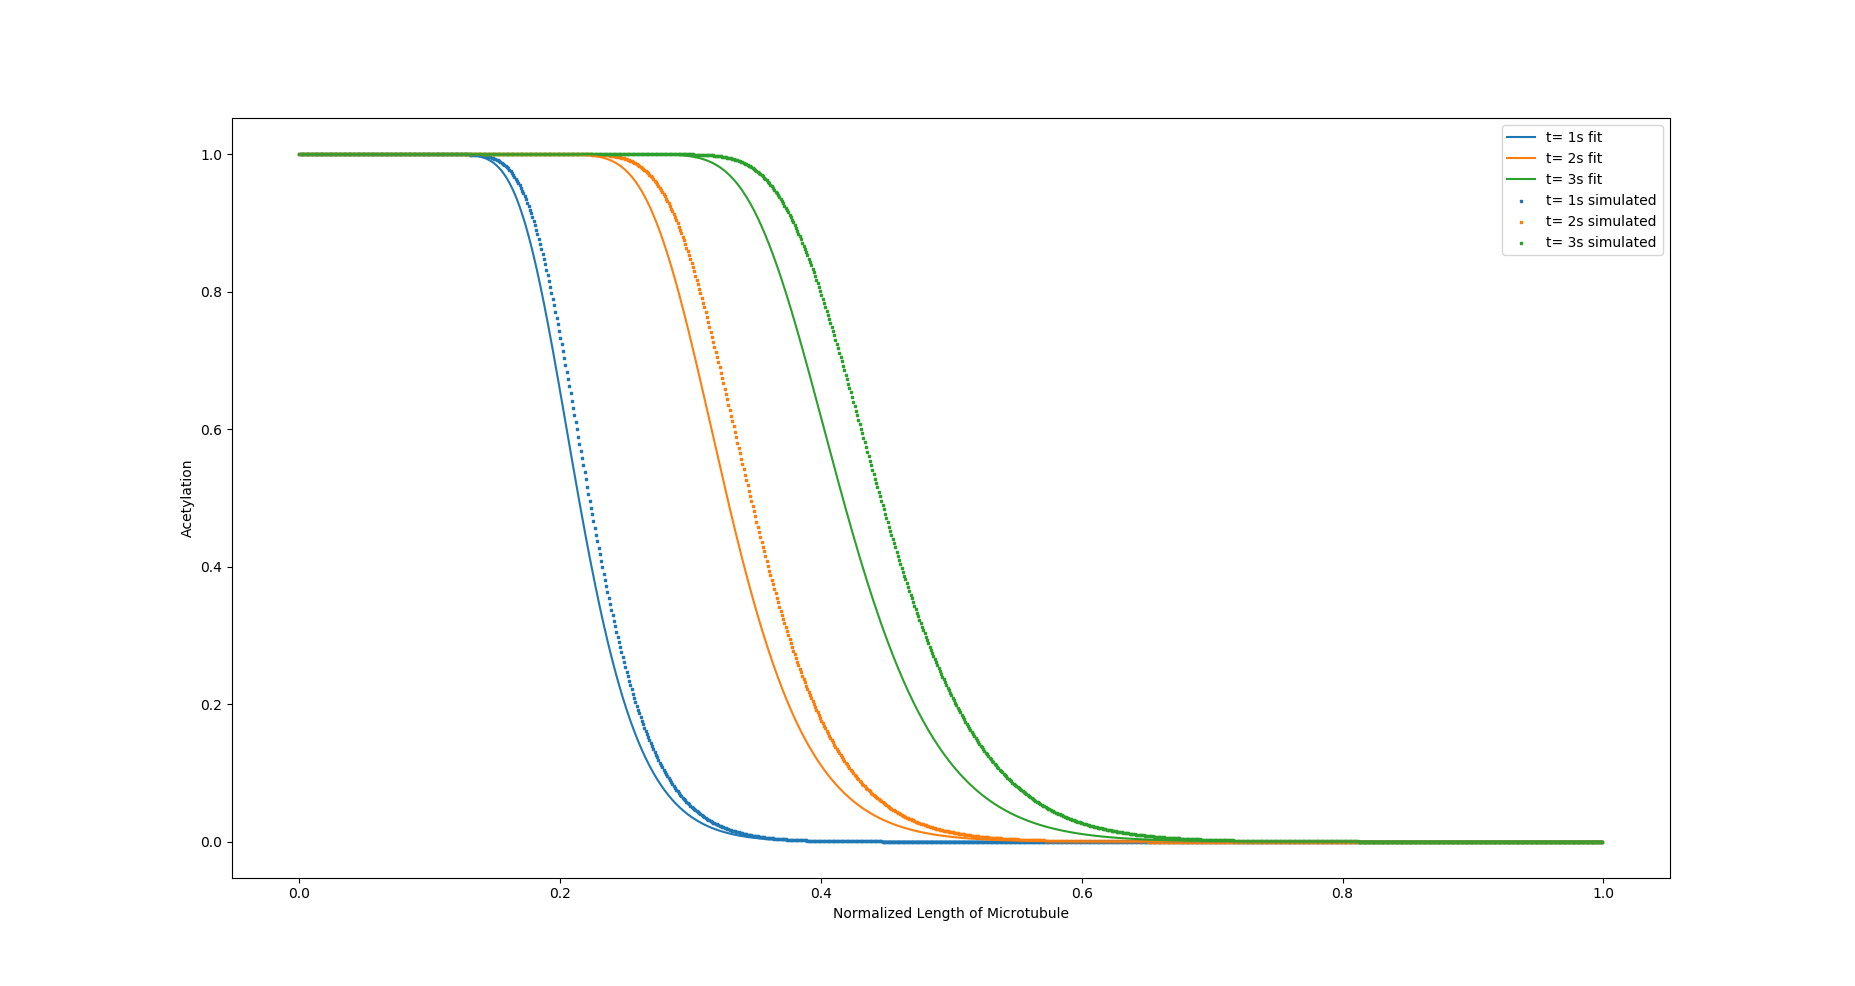
\includegraphics[width=\textwidth]{AcetylationFitsWithSteadyStateMultiplication}
The above two plots use the fits that are provided in the science reports paper as follows:

Occupation Fit:
\begin{equation}
\rho (x,t) = \rho_0 erfc(\frac{x}{\sqrt{4Dt}})
\end{equation}
Acetylation Fit:
\begin{equation}
a(x,t) = 1-exp(-\rho_0\Gamma t ( (1+2z^2)erfc(z) - 2z exp(-z^2)/\sqrt{\pi}))
\end{equation}
where $$ z = \frac{x}{\sqrt{4Dt}} $$

Below are the residuals for each of these fits

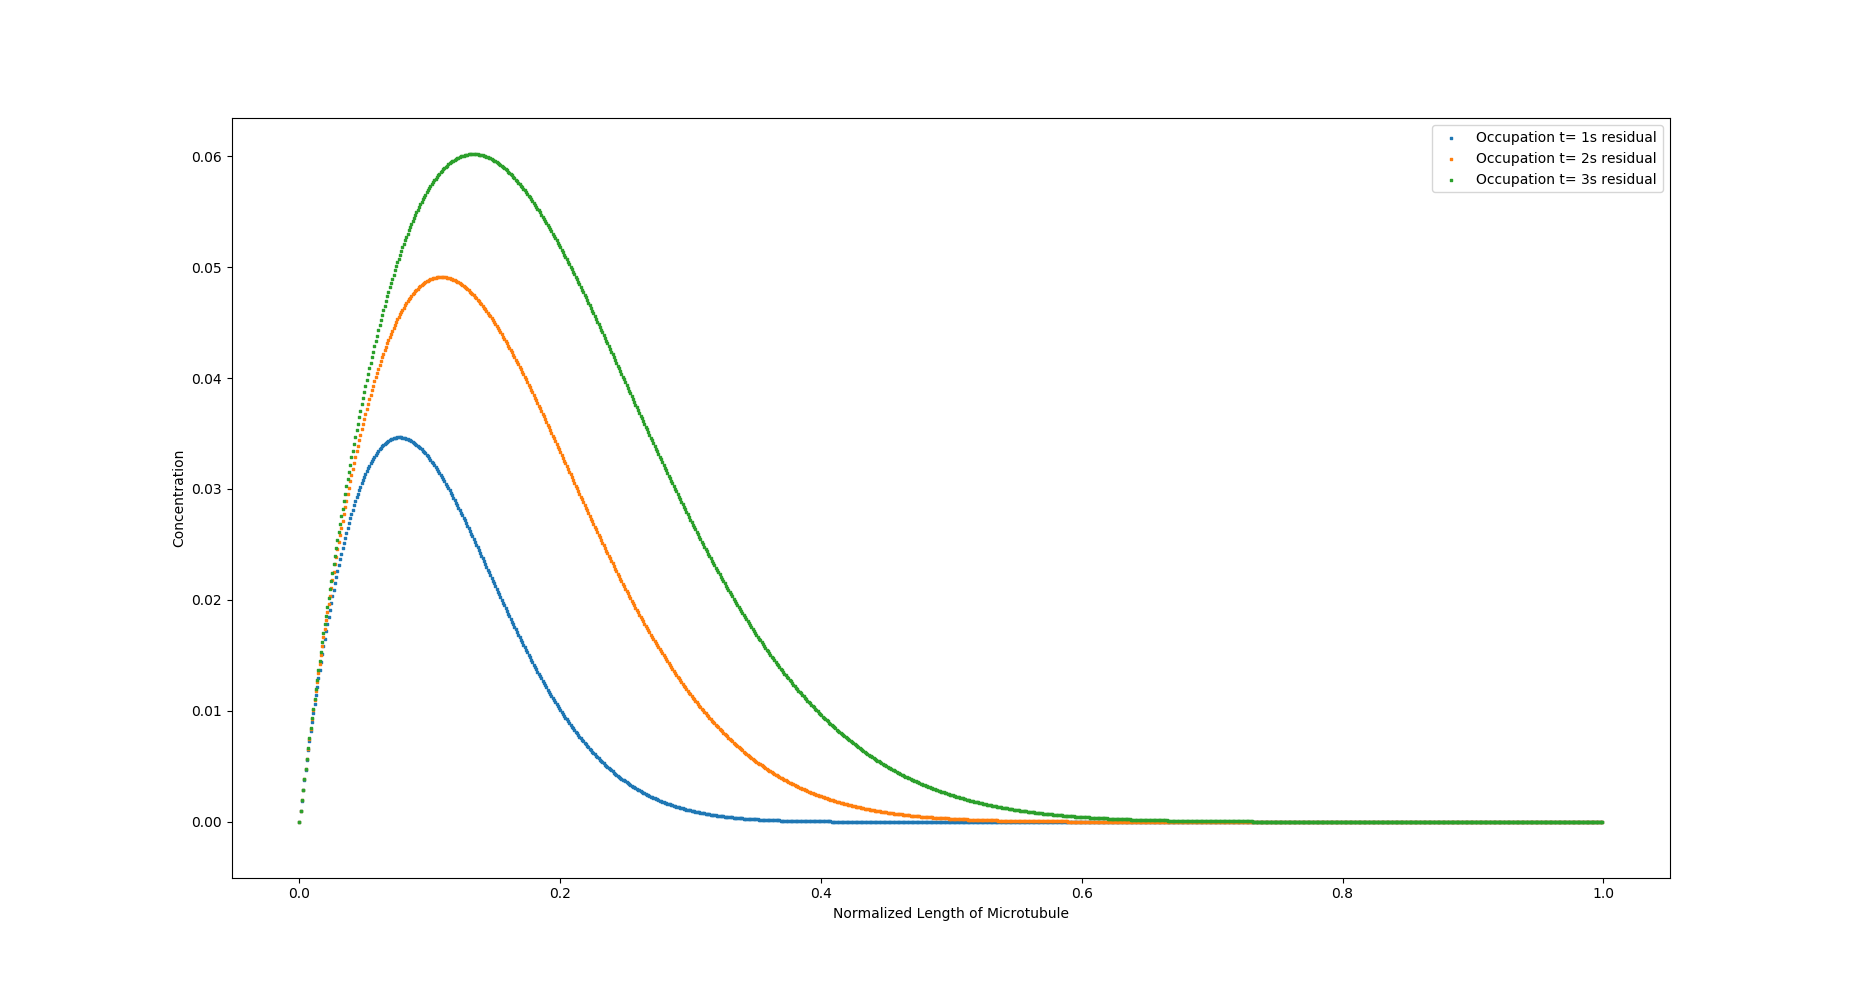
\includegraphics[width=\linewidth]{OccupationSteadyStateMultiplicationResidual}
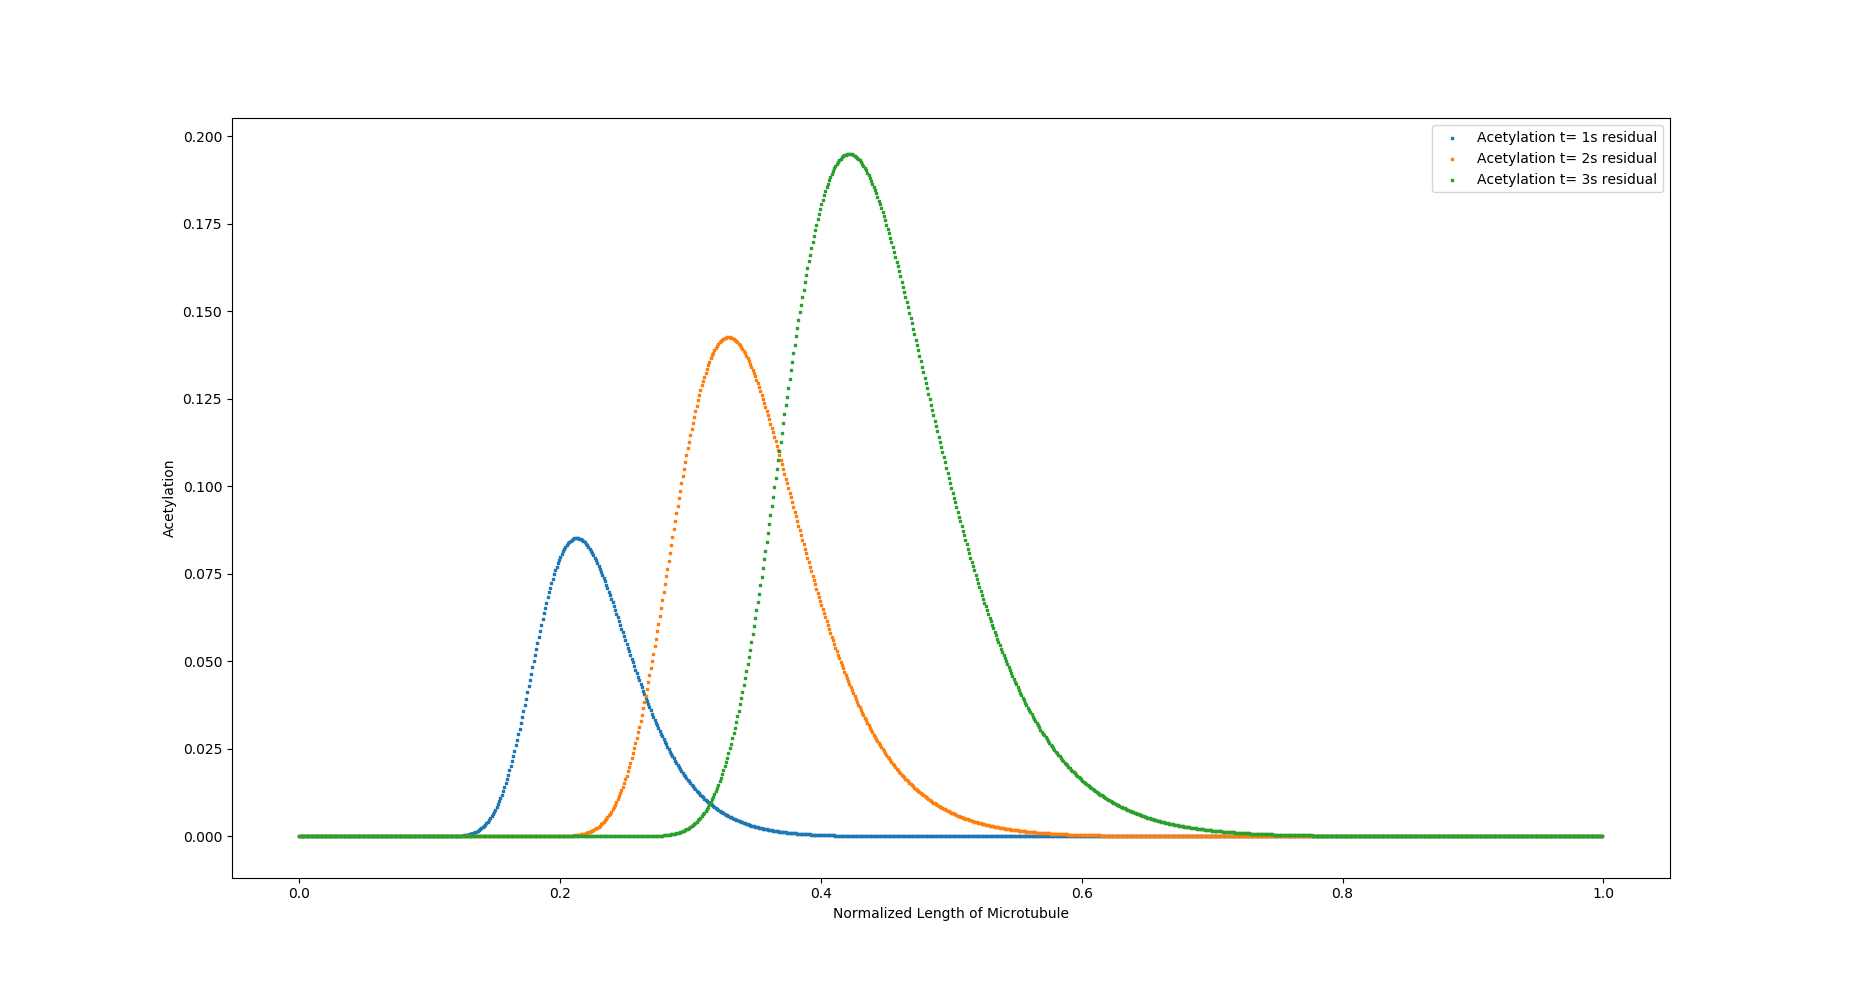
\includegraphics[width=\linewidth]{AcetylationSteadyStateMultiplicationResidual}

Next I looked at what happened if I just didn't have the $\rho_0$ terms within the fits.

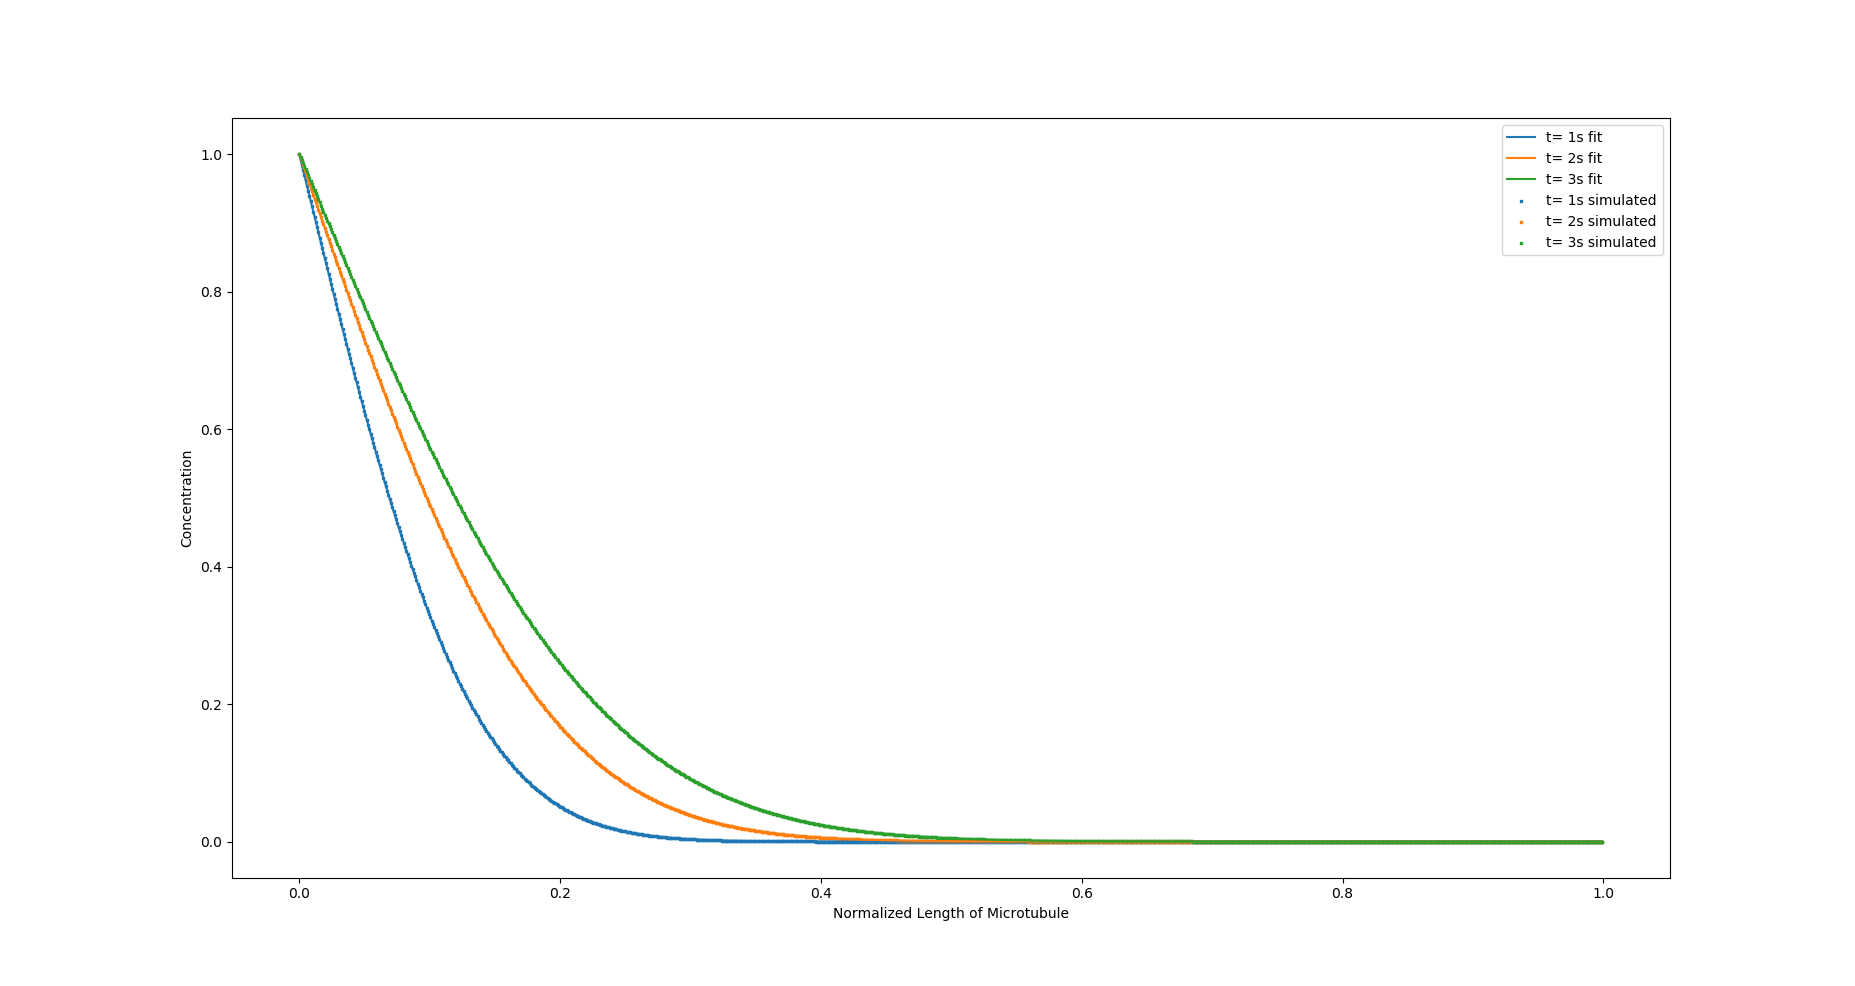
\includegraphics[width=\linewidth]{OccupationFitsNoSteadyStateMultiplication}
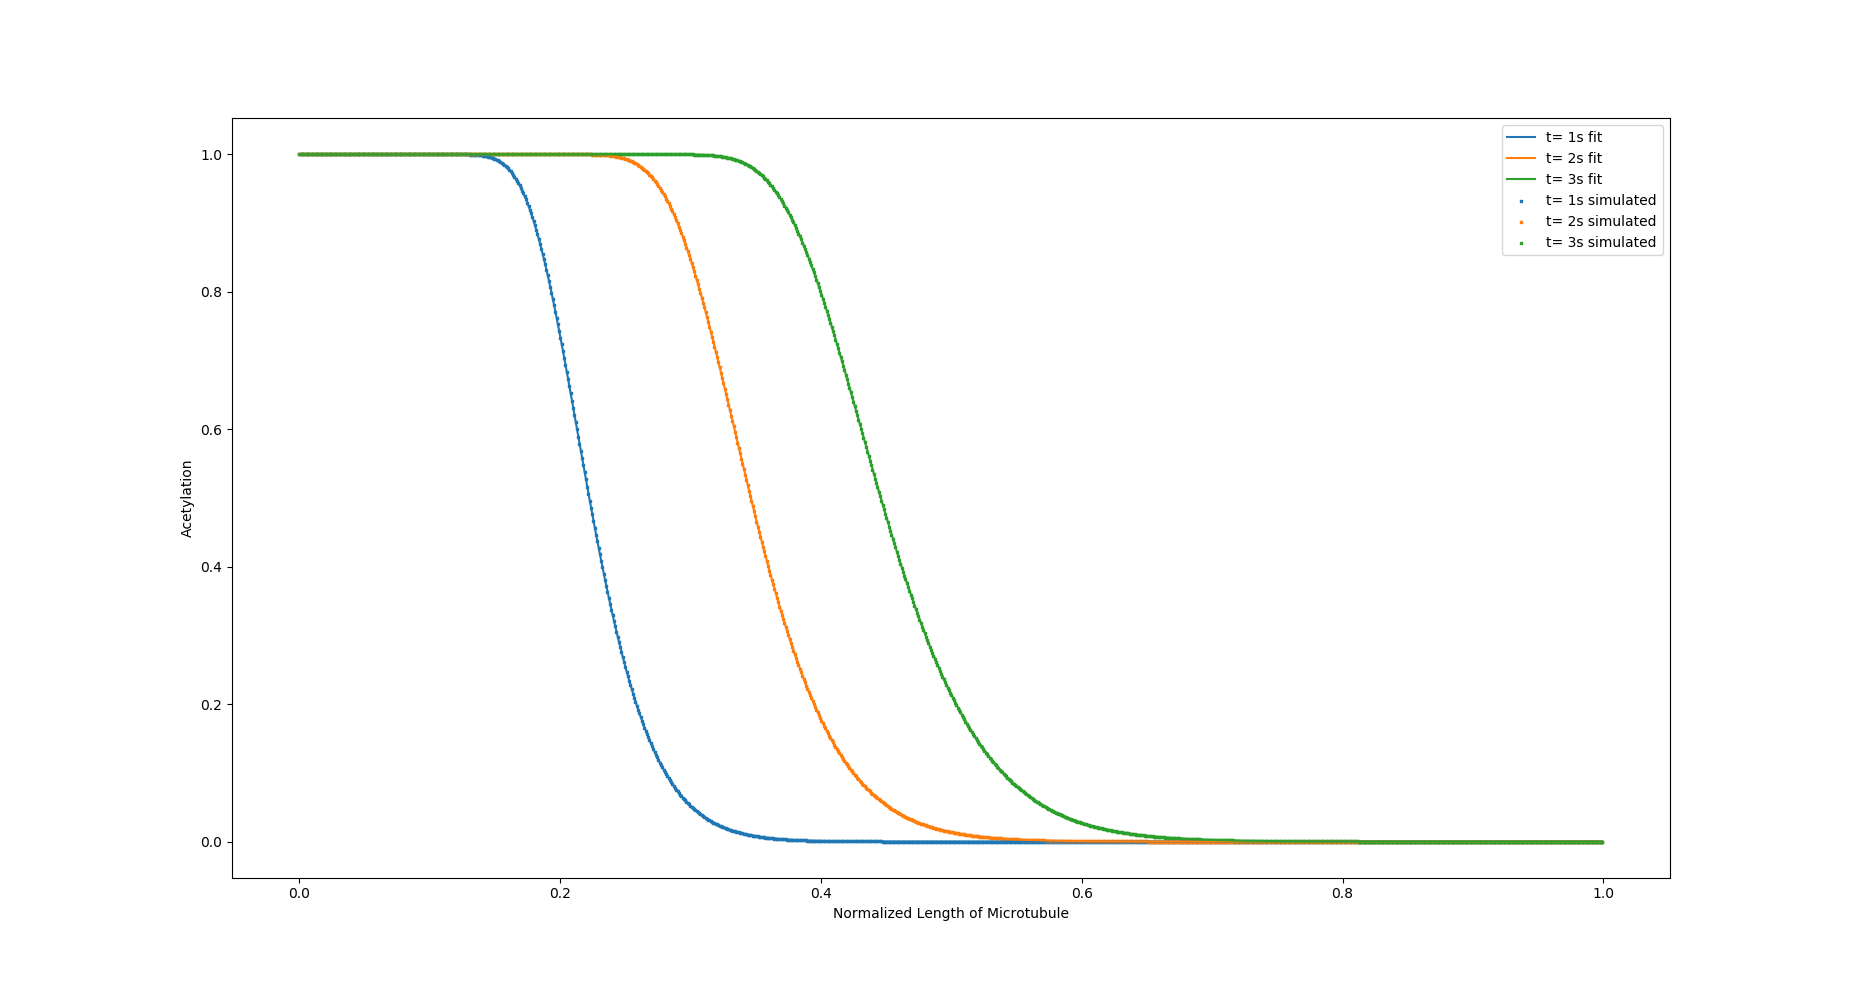
\includegraphics[width=\linewidth]{AcetylationFitsWithoutSteadyStateMultiplication}
The above two plots use the fits that are provided in the science reports paper without the $\rho_0$ multiplication in the fits, where $\rho_0$ is the expected steady state of the system.

Occupation Fit:
\begin{equation}
\rho (x,t) =  erfc(\frac{x}{\sqrt{4Dt}})
\end{equation}
Acetylation Fit:
\begin{equation}
a(x,t) = 1-exp(-\Gamma t ( (1+2z^2)erfc(z) - 2z exp(-z^2)/\sqrt{\pi}))
\end{equation}
Below are the residuals for each of the above two plots

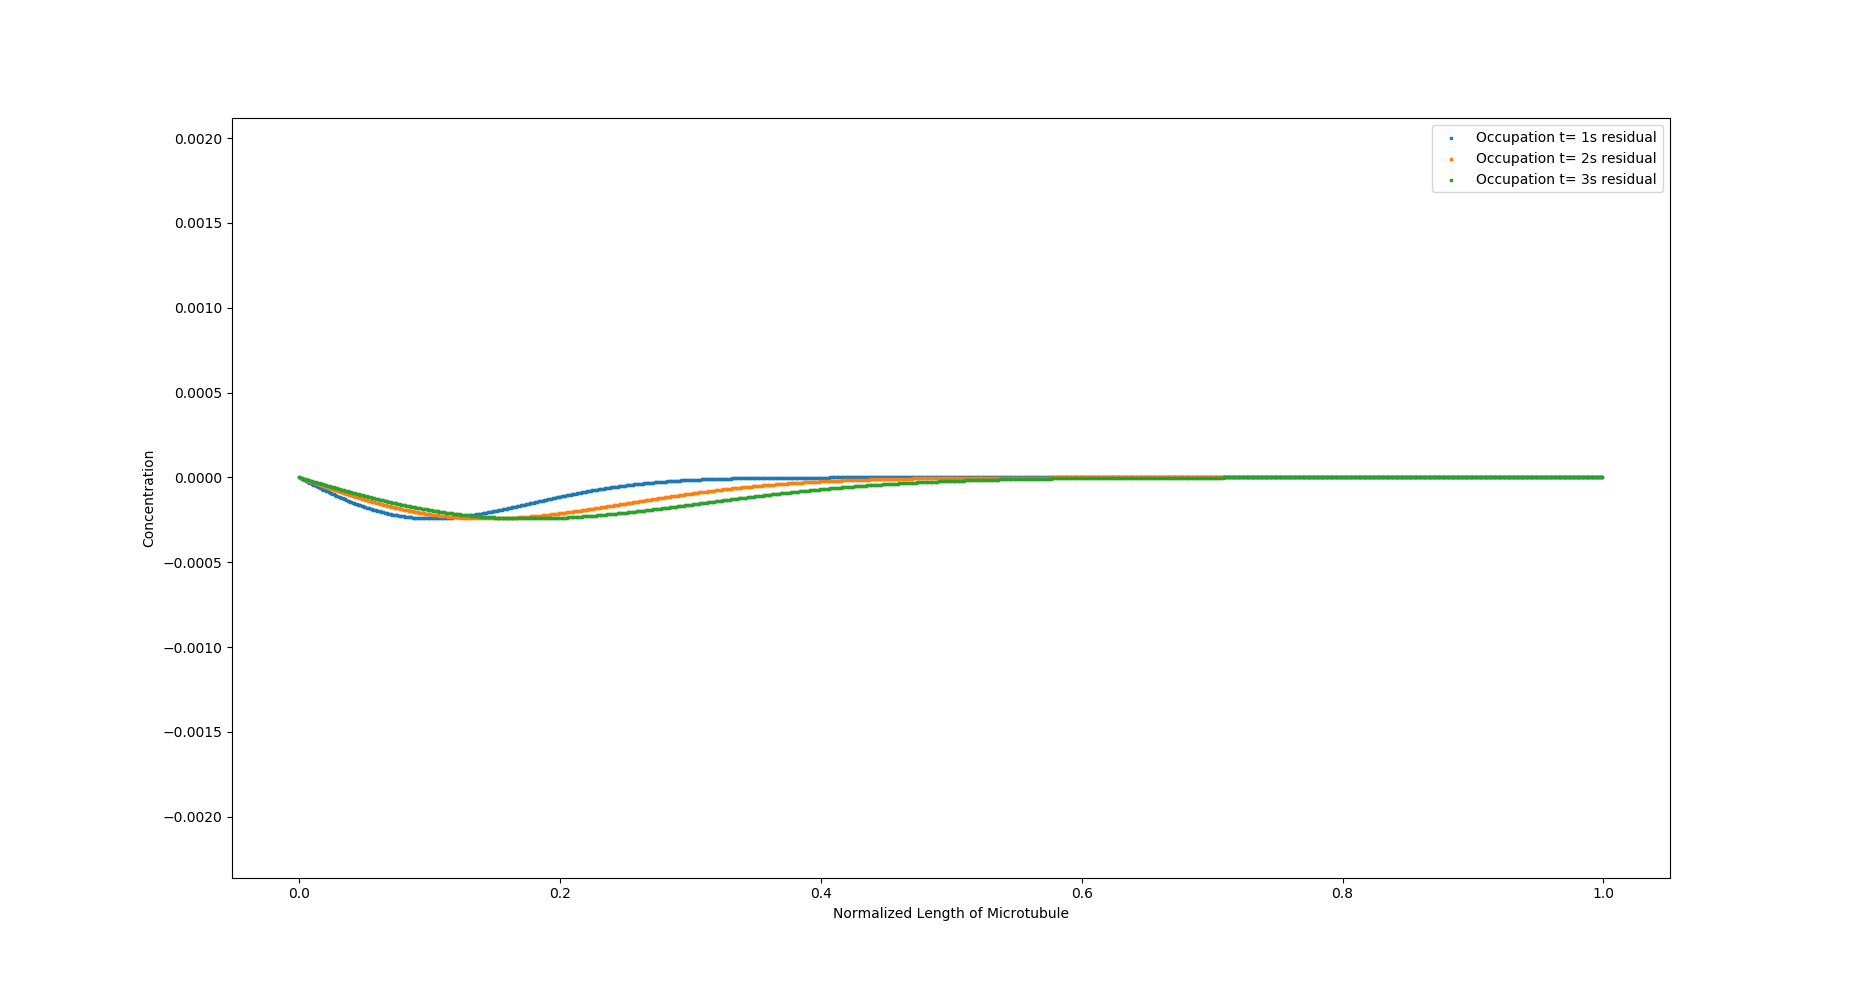
\includegraphics[width=\linewidth]{OccupationNoSteadyStateMultiplicationResidual}
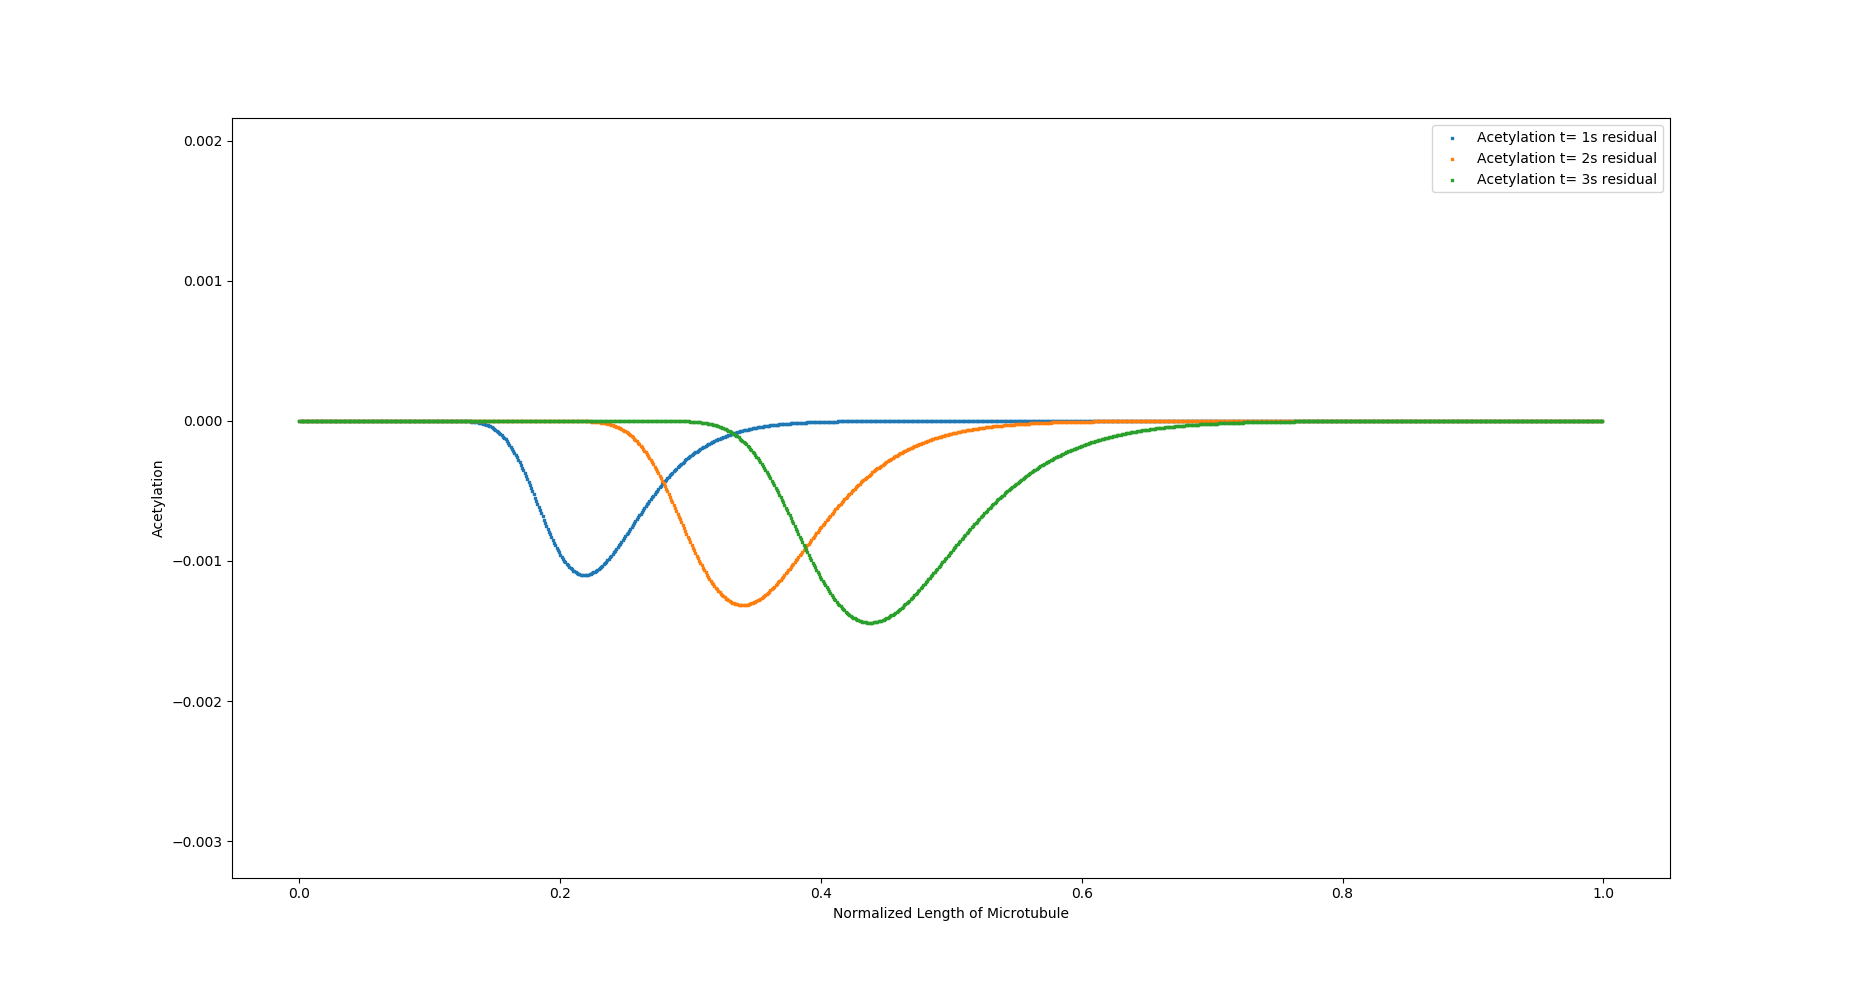
\includegraphics[width=\linewidth]{AcetylationNoSteadyStateMultiplicationResidual}

The shapes in the residuals are similar albeit flipped in sign, however also much smaller.

The final plot I have to show you is the Total Concentration and Acetylation as a function of time.

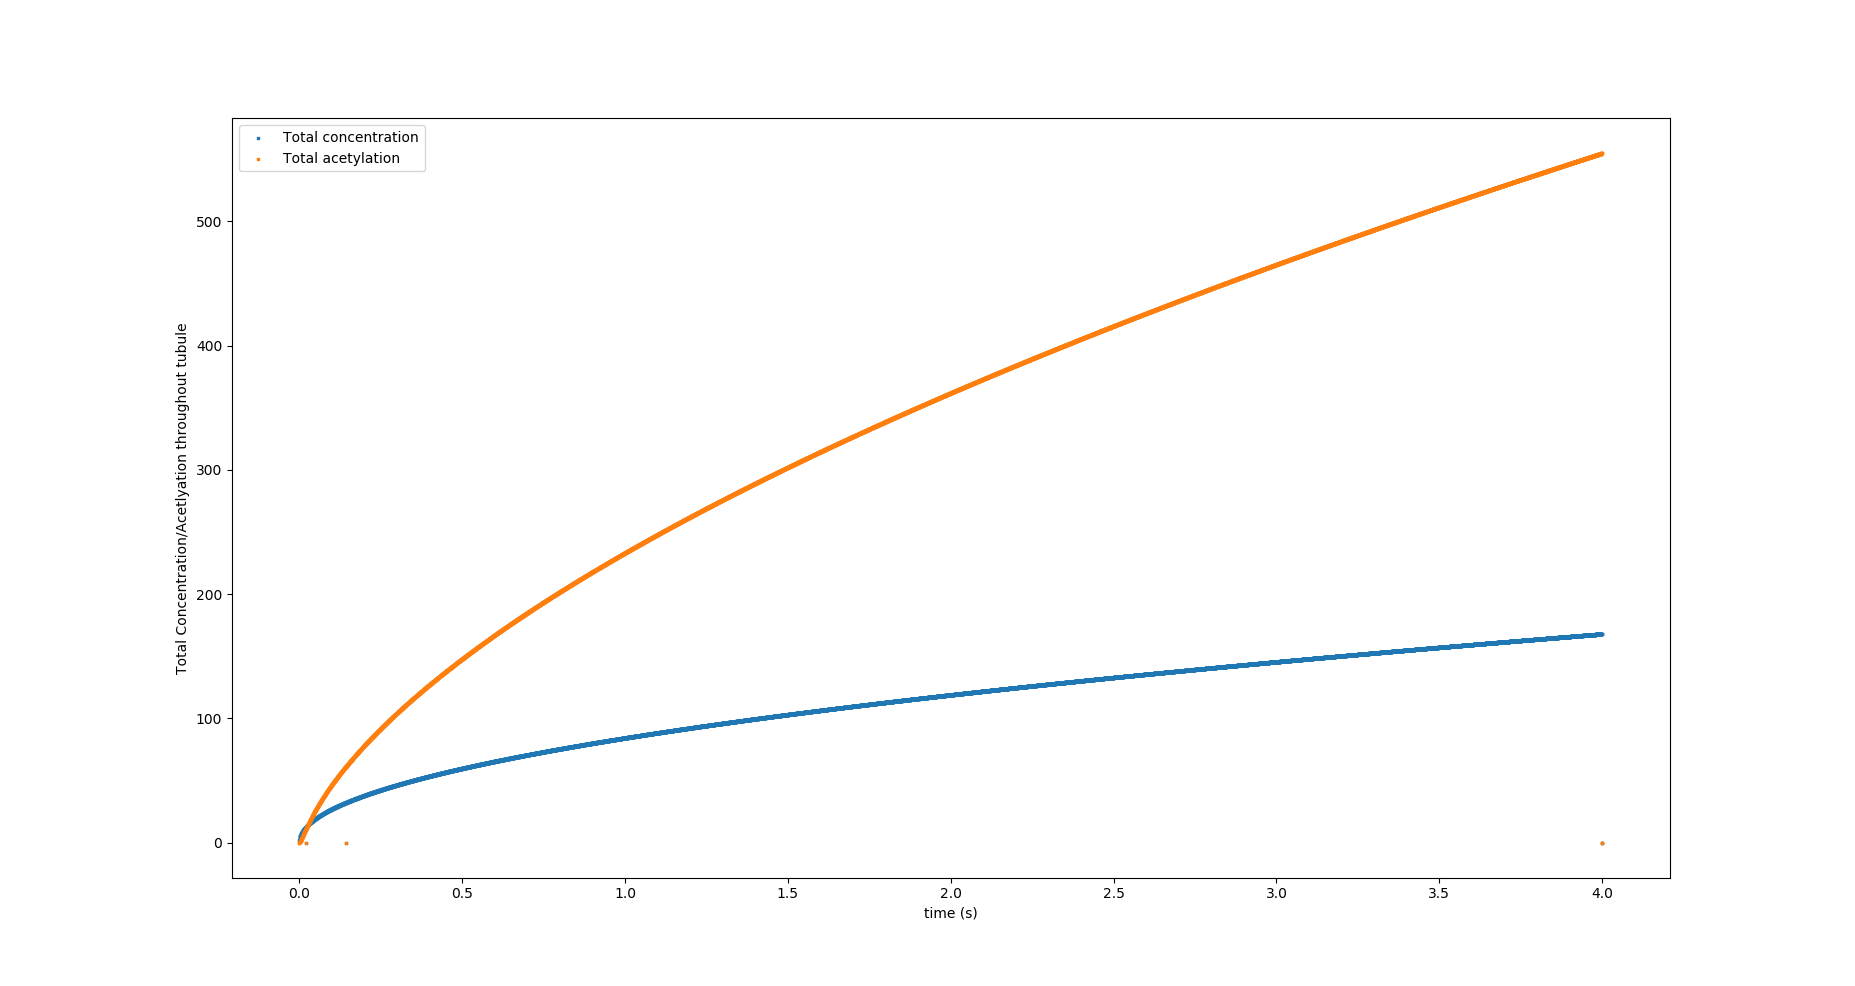
\includegraphics[width=\linewidth]{TotalConcentrationandAcetylationasFunctionofTime}

The tube is discretized into 1024 sites in this case, so if every site was fully acetylated we'd expect the total acetylation to go to 1024. The simulation ran for 4 seconds but I only plotted at 1, 2 and 3 seconds. 

One last thing to mention is that Single File Effects are implemented and I am running this with a large $\rho_{scale}$ so that we recover the $D=D_0$ effect.

If $\frac{d\tilde{t}}{d\tilde{x}^2} > 0.5$
\end{document}          
